%%%%%%%%%%%%%%%%%%%%%%%%%%%%%%%%%%%%%%%%%
% Journal Article
% LaTeX Template
% Version 1.4 (15/5/16)
%
% This template has been downloaded from:
% http://www.LaTeXTemplates.com
%
% Original author:
% Frits Wenneker (http://www.howtotex.com) with extensive modifications by
% Vel (vel@LaTeXTemplates.com)
%
% License:
% CC BY-NC-SA 3.0 (http://creativecommons.org/licenses/by-nc-sa/3.0/)
%
%%%%%%%%%%%%%%%%%%%%%%%%%%%%%%%%%%%%%%%%%

%----------------------------------------------------------------------------------------
%	PACKAGES AND OTHER DOCUMENT CONFIGURATIONS
%----------------------------------------------------------------------------------------

\documentclass[twoside,twocolumn,10pt]{article}

\usepackage{babel}[it]

\usepackage[T1]{fontenc} % Use 8-bit encoding that has 256 glyphs
\usepackage{microtype} % Slightly tweak font spacing for aesthetics

\usepackage[hmarginratio=1:1,top=32mm, left=20mm, right=20mm,columnsep=20pt]{geometry} % Document margins
\usepackage[hang, small,labelfont=bf,up,textfont=it,up]{caption} % Custom captions under/above floats in tables or figures
\usepackage{booktabs} % Horizontal rules in tables

\usepackage{enumitem} % Customized lists
\setlist[itemize]{noitemsep} % Make itemize lists more compact

\usepackage{abstract} % Allows abstract customization
\renewcommand{\abstractnamefont}{\normalfont\bfseries} % Set the "Abstract" text to bold
\renewcommand{\abstracttextfont}{\normalfont\small\itshape} % Set the abstract itself to small italic text

\usepackage{titlesec} % Allows customization of titles
\renewcommand\thesection{\Roman{section}} % Roman numerals for the sections
\renewcommand\thesubsection{\roman{subsection}} % roman numerals for subsections
\titleformat{\section}[block]{\large\scshape\centering}{\thesection.}{1em}{} % Change the look of the section titles
\titleformat{\subsection}[block]{\large}{\thesubsection.}{1em}{} % Change the look of the section titles

\usepackage{fancyhdr} % Headers and footers
\pagestyle{fancy} % All pages have headers and footers
\fancyhead{} % Blank out the default header
\fancyfoot{} % Blank out the default footer
\fancyhead[C]{Progetto di Ingegneria Informatica $\bullet$ Post-Quantum Cryptography} % Custom header text
\fancyfoot[RO,LE]{\thepage} % Custom footer text

\usepackage{titling} % Customizing the title section

\usepackage{hyperref} % For hyperlinks in the PDF

\usepackage{amsmath}

\usepackage{dsfont} % For \mathds commands

\usepackage{graphicx}

\usepackage{mathtools}

\usepackage{booktabs}

\usepackage{pgfplots}

\DeclarePairedDelimiter\ceil{\lceil}{\rceil}
\DeclarePairedDelimiter\floor{\lfloor}{\rfloor}

\usepackage[ruled,vlined,linesnumbered]{algorithm2e}
%----------------------------------------------------------------------------------------
%	TITLE SECTION
%----------------------------------------------------------------------------------------

\setlength{\droptitle}{-4\baselineskip} % Move the title up

\bibliographystyle{ieeetr}


\pretitle{\begin{center}\Huge\bfseries} % Article title formatting
\posttitle{\end{center}} % Article title closing formatting
\title{Progetto di Ingegneria Informatica \\ Post-Quantum Cryptography} % Article title
\author{%
\textsc{Domenico Cacace} \\[1ex] % Your name
\small{Matricola 891291} \\
}
\date{} % Leave empty to omit a date
\renewcommand{\maketitlehookd}{%
\begin{abstract}
In questa relazione analizziamo l'algoritmo di inversione polinomiale proposto da D.J. Bernstein e B.Y. Yang, focalizzandoci in particolare su una sua implementazione
per polinomi binari intesa per l'utilizzo all'interno di un crittosistema resistente ad attacchi di computer quantistici; passiamo quindi ad analizzare
le criticità dell'implementazione, fornendo alcuni metodi per migliorare questi aspetti. Infine, valutiamo le performance e le proprietà dell'algoritmo comparandole
con altri algoritmi per il medesimo scopo.

\end{abstract}
}

%----------------------------------------------------------------------------------------

\begin{document}

% Print the title
\maketitle

\section{Introduzione}
L' interesse per la ricerca nel campo della crittografia post-quantistica è cresciuto esponenzialmente
con l'annuncio del National Institute of Standards and Technology dell'avvio del processo di valutazione
e standardizzazione di uno o più algoritmi di crittografia asimmetrici resistenti ad attacchi di computer 
quantistici.\footnote{\href{https://csrc.nist.gov/projects/post-quantum-cryptography}{https://csrc.nist.gov/projects/post-quantum-cryptography}};
tra i candidati troviamo LEDAcrypt\cite{baldi2019ledacrypt, ledaKEM}, basato sul crittosistema McEliece.\\
I crittosistemi basati sulla teoria dei codici hanno lo svantaggio di usare chiavi pubbliche piuttosto larghe; un modo per ridurre le dimensioni
di queste chiavi è utilizzare famiglie di codici che consentono di essere rappresentati in modo più efficiente per quanto riguarda lo spazio occupato,
come ad esempio i codici QC-MDPC (Quasi-cyclic moderate-density parity-check): questi codici sono composti da matrici a blocchi quadrate circolanti,
dove ogni riga è ottenuta dallo shift circolare della precedente. L'aritmetica di queste matrici di dimensioni $p \times p$ è isomorfa a quella dei polinomi modulo
$x^p-1$, per cui possiamo sfruttare questa proprietà per ridurre il tempo di esecuzione del calcolo dell'inverso.

\section{Analisi dell'algoritmo}
L'algoritmo proposto in~\cite{bernstein2019fast} è basato su un approccio \textit{divide et impera}: l'operando viene diviso dalla funzione
\texttt{jumpdivstep}, che prende in input due polinomi $f, g$, di grado al più $n$ e con $\delta = \deg{f} - \deg{g}$ e individua
un \textit{pivot} $j$, che divide i polinomi a metà. La funzione \texttt{jumpdivstep} è quindi chiamata ricorsivamente passando come parametri le due 
metà dei polinomi appena individuate, finché la loro dimensione non è sufficientemente piccola (vedi~\ref{impl}); questo punto viene invocata la 
funzione \texttt{divstep}, che gestisce il caso base della ricorsione. 
La funzione \texttt{jumpdivstep} prende come input di partenza la rappresentazione riflessa di modulo $f(x)$ ed elemento da invertire $a(x)$, e ritorna alla fine
 la rappresentazione riflessa dell'inverso di $a(x)$, $\mathcal{H}_{0,1}$, con $V(x) \equiv a^{-1}(x)$.

 \begin{algorithm}
    \small
    \SetAlgoLined
    \BlankLine
    \SetKwFunction{jumpdivstep}{jumpdivstep}
    \SetKwFunction{invert}{invert}

    \SetKwFunction{divstep}{divstep}
    \SetKwProg{Fn}{function}{:}{}
    \Fn{\jumpdivstep{$n, \delta, f(x), g(x)$}}{

    \If{$n \leq ws$}{
        \Return\texttt{divstep($n, \delta, f(x), g(x)$)\;}
    }

        $j \leftarrow \lfloor \frac{n}{2} \rfloor$\;
        $\delta, \mathcal{P} \leftarrow$ \texttt{jumpdivstep}($j, \delta, f(x)\mod x^j, g(x)\mod x^j$)\;
        $f^{\prime}(x) \leftarrow \mathcal{P}_{0,0}\cdot f(x) + \mathcal{P}_{0,1}\cdot g(x)$\;
        $g^{\prime}(x) \leftarrow \mathcal{P}_{1,0}\cdot f(x) + \mathcal{P}_{1,1}\cdot g(x)$\;
        $\delta, \mathcal{Q} \leftarrow$ \texttt{jumpdivstep}($n-j, \delta, \frac{f^{\prime}(x)}{x^j}, \frac{g^{\prime}(x)}{x^j}$)\;

        \Return$\delta, (\mathcal{P}\times\mathcal{Q})$
    }
    \BlankLine
    \Fn{\invert{$f(x), a(x)$}}{
        $S(x) \leftarrow$ \texttt{MIRROR}($f(x)$)\;
        $R(x) \leftarrow$ \texttt{MIRROR}($a(x)$)\;
        $\delta, \mathcal{H} \leftarrow$ \texttt{jumpdivstep}($2m - 1, 1, S(x), R(x)$)\;
        $V(x) \leftarrow$ \texttt{MIRROR}($\mathcal{H}_{0,1}$)\;
        \Return$V(x)$\;

    }

     \caption{jumpdivstep}
    \end{algorithm}
    \subsection*{\textbf{\textit{Simulazione} dell'algoritmo}} Possiamo, partendo dall'algoritmo qui presentato, ricostruire un albero di ricorsione tracciando tutte le
    chiamate ed i vari parametri necessari: la prima chiamata a \texttt{jumpdivstep} (riga 14) è la radice dell'albero, 
    la prima chiamata effettuata (riga 6) corrisponde al figlio destro di un nodo, mentre la seconda (riga 9) corrisponde al
    figlio sinistro; quando la dimensione degli operandi è pari o inferiore alla \textit{word size}, ossia quando viene 
    invocata la funzione \texttt{divstep}, il nodo corrispondente nell'albero di ricorsione risulta essere una foglia.
    
    Analizzando l'albero di ricorsione ed i parametri relativi ai nodi, possiamo inoltre determinare le dimensioni
    dei vettori che contengono i risultati intermedi ($\mathcal{P}, \mathcal{Q}$) e gli operandi intermedi
    ($f^{\prime}(x), g^{\prime}(x)$), nonché gli indici di accesso ai suddetti per ogni chiamata. Da qui, possiamo \textit{simulare}
    le chiamate attraversando l'albero usando un approccio \textit{depth-first}, dando priorità ai figli destri
    (che per costruzione corrispondono alla prima chiamata). 
    È inoltre interessante notare che le operazioni ed i parametri necessari per ogni chiamata dipendano solo dalla 
    dimensione dei parametri di input, e non dai parametri stessi; questo ci permetterà di effettuare tutte le ottimizzazioni
    riportate in~\ref{ott}, e quindi poter generare una versione
    iterativa di \texttt{jumpdivstep} specifica per dimensione dell'input.

    \subsubsection*{Contenuto dei nodi}
    Ad ogni nodo dell'albero di ricorsione corrisponde una chiamata a \texttt{jumpdivstep}, ognuna caratterizzata
    dai propri parametri, tra cui:
    \begin{itemize}
        \item \texttt{n}: grado massimo dei operandi ricevuti in input
        \item \texttt{j}: grado massimo degli operandi passati alla prima chiamata ricorsiva (figlio destro)
        \item \texttt{n-j}: grado massimo degli operandi passati alla seconda chiamata ricorsiva (figlio sinistro)
        \item \texttt{num\_digits\_(n|j|nminusj)}: numero di \texttt{DIGIT} (vedi~\ref{impl}) necessari a contenere gli operandi di cui sopra
    \end{itemize}



\section{Implementazione ed Ottimizzazione}\label{impl}
\subsection*{\textbf{Rappresentazione dei polinomi}}
I polinomi, elementi dell'anello $GF(2)[x]$, sono salvati in forma binaria compatta: ogni bit in un byte rappresenta un 
coefficiente di un polinomio binario in formato Big-Endian (leggendo da sinistra a destra, i primi elementi che
si incontrano sono i coefficienti di grado più alto)

Una \textit{machine word} è considerata un \texttt{digit} ed i byte che
compongono un \texttt{digit} sono in formato Big Endian; allo stesso modo, 
anche gli elementi con più \texttt{digit} sono rappresentati in 
formato Big Endian.
\begin{table}
    \caption{Rappresentazione dei polinomi, singolo byte}
    \begin{tabular}{lll}
    \hline
    \textbf{Bin} & \textbf{Hex} & \textbf{Polinomio} \\
    \hline
    0000 0000 & 0x00 & 0 \\
    0000 0001 & 0x01 & 1 \\
    0000 0002 & 0x02 & $x$ \\
    0000 0003 & 0x03 & $x+1$ \\
    $\cdots$ & $\cdots$ & $\cdots$ \\
    0000 1111 & 0x0F & $x^3+x^2+x+1$ \\
    $\cdots$ & $\cdots$ & $\cdots$ \\
    1111 1111 & 0xFF & $x^7+x^6+x^5+\cdots+x+1$ \\
    \hline
    \end{tabular}
\end{table}
\subsubsection*{Estensioni dell'ISA x86}
L'implementazione proposta in~\cite{benchmark} utilizza AVX, un'estensione 
dell' Instruction Set Architecture di x86 che permette di lavorare su più parole di memoria
in parallelo, portando notevoli vantaggi nelle operazioni aritmetiche: ciò significa,
su una macchina a 64 bit (dimensione di un \texttt{digit}), lavorare su 128 o 256 bit.
Questo ci permette inoltre di avere un'implementazione molto efficiente per i prodotti, utilizzando funzioni
altamente specializzate per polinomi di 8 \texttt{digit} o meno e loro combinazioni per dimensioni
maggiori, come riportato in~\cite{bodrato2007towards}; gli intrinsics, funzioni gestite direttamente dal compilatore che permettono di usare
istruzioni specifiche dell'architettura per cui si sta compilando come fossero chiamate a funzioni standard, permettono inoltre 
l'implementazione delle diverse versioni di \texttt{divstep}.



\subsection*{\textbf{Punti critici}}\label{crit}
Tramite un'analisi di complessità asintotica, supportata dai risultati sperimentali ottenuti tramite \texttt{callgrind}, notiamo che la 
maggior parte del tempo di esecuzione è dovuta a \texttt{gf2x\_scalarprod}: ciò non ci sorprende, in quanto
questa funzione è invocata due volte per il calcolo di $\bar{f(x)}$ e $\bar{g(x)}$ (\texttt{jumpdivstep}, righe 7-8), e altre quattro per $P \times Q$ (\texttt{jumpdivstep}, riga 10); inoltre,
per quest'ultima operazione, sono necessarie altrettante chiamate a \texttt{memcpy}, per spostare i risultati ottenuti da un vettore temporaneo alla
destinazione desiderata.
\begin{algorithm}
    \small
    \SetAlgoLined
    \SetKwFunction{scalarprod}{scalarprod}    
    \KwIn{$a_0, a_1, b_0, b_1$: array di polinomi\newline
                $na, nb$: dimensioni degli array di polinomi}
    \KwOut{$res = a_0\cdot b_0 + a_1 \cdot b_1$, dimensione $na+nb$}
    \BlankLine
    \SetKwProg{Fn}{function}{:}{}

    \Fn{\scalarprod{$na, a_0, a_1, nb, b_0, b_1$}}{

        \texttt{DIGIT} tmp[$na*2$]\;
        \texttt{DIGIT} tmp2[$na*2$]\;
        \texttt{DIGIT} buffer[$na$]\;
        \texttt{memset}(buffer, 0x00, ($na-nb$)*\texttt{DIGIT\_SIZE\_B})\;
        \BlankLine
        \texttt{memcpy}(buffer+($na-nb$), $b_0$, $nb$*\texttt{DIGIT\_SIZE\_B})\;
        \texttt{GF2X\_MUL}($na*2$, tmp, $a_0$, buffer)\;
        \BlankLine
        \texttt{memcpy}(buffer+($na-nb$), $b_1$, $nb$*\texttt{DIGIT\_SIZE\_B})\;
        \texttt{GF2X\_MUL}($na*2$, tmp2, $a_1$, buffer)\;
        \BlankLine
        \texttt{gf2x\_add}($na*2$, tmp, tmp, tmp2)\;
        \texttt{memcpy}(res, tmp+($na-nb$), ($na+nb$)*\texttt{DIGIT\_SIZE\_B})\;
        \Return{res}
    }
    \caption{\texttt{gf2x\_scalarprod} (per $na > nb$)}
    \end{algorithm}

La funzione \texttt{gf2x\_scalarprod} prende in input due coppie di polinomi ($a_{0},a_{1}$, $b_{0},b_{1}$), di dimensione rispettivamente $na$ e $nb$ \texttt{digit}, e 
produce in output il prodotto scalare $res = a_{0} \cdot b_{0} + a_{1} \cdot b_{1}$, di dimensione $nr = na+nb$; in realtà, per poter eseguire le moltiplicazioni
tra polinomi, è necessario spostare l'operando più corto in un buffer (righe 6, 8) e aggiungere zeri nelle posizioni dei coefficienti più significativi mancanti (riga 5), fino
a raggiungere la dimensione dell'altro operando. 

Una volta calcolati i prodotti, questi vengono ulteriormente manipolati, troncando i coefficienti superflui, shiftandoli (\texttt{jumpdivstep}, righe 7-8) e 
spostandoli da una posizione all'altra; analizzando come questi polinomi vengono manipolati, possiamo andare a salvare i risultati direttamente nelle posizioni
corrette, riduendo i tempi di esecuzione.

\subsection*{\textbf{Ottimizzazioni}}\label{ott}

\subsubsection*{Allocazione dei polinomi}
Il primo passo nell'unrolling dell'algoritmo ricorsivo consiste nell'allocare in una volta sola tutta la memoria necessaria per salvare
i risultati e gli operandi intermedi, ossia $ P, Q, \bar{f(x)}$ e $\bar{g(x)}$; le stesse porzioni di memoria vengono riutilizzate da diverse
chiamate in momenti diversi, per cui viene presa la dimensione massima per ogni \textit{slot}, individuabile percorrendo il ramo destro dell'albero di ricorsione
dalla radice all'ultima foglia. Partendo con operandi di grado $n_0-1$, \texttt{digit} di dimensione $s$ e parole di memoria di dimensione $ws$
(entrambe espresse in bit), avremo un albero di ricorsione di profondità $d=\lceil \log_{2}\frac{n}{s} \rceil$; per ogni livello, avremo 
\begin{equation*}
    j_{i} = \floor*{\left(\floor*{\frac{n_i}{2}} + ws - 2\right) \cdot \frac{1}{ws-1}} \cdot (ws-1)
\end{equation*}
\begin{equation*}
    n_{i} = j_{i-1} \qquad (i \neq 0)
\end{equation*}
Le operazioni di somma, prodotto e divisione che includono $ws$ sono necessarie ad ottenere, alla fine della ricorsione, polinomi di grado $ws-1$\footnote{In alcuni casi 
i polinomi ottenuti sono di grado inferiore per \textit{mancanza di coefficienti}}, in modo da sfruttare appieno gli intrinsics di AVX.

Partendo da quanto appena trovato, possiamo calcolare il numero di \texttt{digit} necessario a memorizzare i vari polinomi:
\begin{equation*}
    \begin{aligned}
    \mathrm{\texttt{num\_digits\_n}_i} = \ceil*{\frac{n_i}{s}}\\
    \mathrm{\texttt{num\_digits\_j}_i} = \ceil*{\frac{j_i}{s}}\\
    \mathrm{\texttt{num\_digits\_nminusj}_i} = \ceil*{\frac{n_i - j_i}{s}}\\
    \end{aligned}
\end{equation*}

Possiamo quindi individuare le dimensioni degli slot dei vari array in base al livello di profondità $i$:
\begin{itemize}
        \item $P$: $d$ slot di dimensione $\mathrm{\texttt{num\_digits\_j}}_i$, 4 array
        \item $P$: $d$ slot di dimensione $\mathrm{\texttt{num\_digits\_nminusj}}_i$, 4 array
        \item $\bar{f(x)}$: $d-1$ slot di dimensione $\mathrm{\texttt{num\_digits\_n}}_i + \mathrm{\texttt{num\_digits\_j}}_i$, 1 array
        \item $\bar{g(x)}$: come al punto precedente.
\end{itemize}
Tenendo traccia delle dimensioni dei vari componenti è poi possibile determinare gli indici di accesso agli array per i vari valori di $d$.

\subsubsection*{Scomposizione dei prodotti}

Come accenato, le funzioni per il calcolo del prodotto tra polinomi richiedono operandi di dimensione uguale: invece di aggiungere coefficienti
nulli al polinomio più corto~($a = 0, a_1$), possiamo dividere il polinomio più lungo ($b = b_0, b_1$) in due parti: 
\begin{center}
    \begin{tabular}{cccc}
            & $0$ & $a_1$ & $\times$ \\
            & $b_0$ & $b_1$ & =\\
            \hline
            & $0\cdot b_1$ &$a_1\cdot b_1$ & +\\
            &\hspace{-9ex}$0\cdot b_0$&\hspace{-9ex}$a_1\cdot b_0$&\hspace{-10ex}\--
    \end{tabular}
\end{center}
la parte \textit{inferiore} ($b_{1}$, coefficienti meno significativi),
della stessa dimensione di $a_1$, viene moltiplicata direttamente con $a_1$ stesso; il procedimento viene quindi ripetuto considerando ora il polinomio $a_1$ e 
la parte restante dell'altro polinomio, $b_{0}$, fino ad esaurimento.


I vari sottoprodotti che vengono calcolati vanno quindi sommati: dati due sottoprodotti successivi $r_i$, $r_{i+1}$, abbiamo che $\deg({r_{i+1}})-\deg({r_i}) = na$
(in modo simile a quanto sopra, $na$ indica la dimensione del poliniomio più corto alla $i$-esima iterazione): con riferimento all'esempio, abbiamo che $r_1 = a_1\cdot b_1$ e $r_2 = a_1\cdot b_0$,
per cui i $na$ coefficienti meno significativi di $r_1$ vengono sommati ai $na$ coefficienti più significativi di $r_2$, mentre i restanti ($na$ per $r_1$, $nb$ per $r_2$) vengono semplicemente riportati 
come sono nel risultato, in quanto i sottoprodotti restanti sono nulli.


Quindi, nell'implementazione del generatore, sostituiamo ogni chiamata a \texttt{gf2x\_scalarprod} con la corrispondente sequenza di \texttt{gf2x\_add} e \texttt{GF2X\_MUL},
utilizzando un accumulatore, $nr$, per tenere traccia dell'offset da considerare;
inoltre, nel caso i due operandi siano di dimensioni inferiori agli 8 \texttt{digit}, andiamo ad utilizzare direttamente le funzioni specifiche per la dimensione
desiderata (\texttt{gf2x\_mul\_X\_avx}), evitando le chiamate a \texttt{GF2X\_MUL}.

\subsubsection*{Troncamento e shift dei risultati}
In quasi tutti i casi l'output di \texttt{gf2x\_scalarprod} viene troncato, eliminando sempre una porzione dei coefficienti più significativi che eccedono la dimensione necessaria; dato che il
metodo di moltiplicazione parte dai coefficienti meno significativi, possiamo bloccarne l'esecuzione prematuramente appena abbiamo tutti i coefficienti
necessari, evitando il calcolo di quelli che sarebbero poi tagliati. Ciò viene banalmente implementato  nel generatore utilizzando lo stesso accumulatore
$nr$ citato al punto prima, ma sottraendovi il numero di \texttt{digit} che sarebbero eliminati successivamente. 

A questo punto, possiamo quindi evitare di utilizzare un vettore ausiliario per il calcolo dei prodotti (\texttt{jumpdivstep}, righe 6-8, 10), ma ne abbiamo ancora bisogno
per il calcolo di $\frac{\bar{f(x)}}{x^{j}}$ e $\frac{\bar{g(x)}}{x^{j}}$: queste divisioni sono infatti ottenute tramite uno shift a sinistra di $j$ bit; per risolvere
questo problema, dividiamo lo shift in due parti:
\begin{itemize}
    \item shift di ($\lfloor\frac{j}{\texttt{DIGIT\_SIZE\_b}}$\footnote{Dimensione di un \texttt{digit} in bit}$\rfloor$) \texttt{digit} interi;
    \item shift di ($j \mod \texttt{DIGIT\_SIZE\_b}$) bit singoli.
\end{itemize}
Lo shift dei \texttt{digit} interi può essere ricondotto al problema del troncamento dei coefficienti più significativi, aggiustando opportunamente gli offset; per quanto riguarda
lo shift dei singoli bit (che saranno per costruzione meno di quelli in un \texttt{digit}), abbiamo bisogno di aggiungere un \texttt{digit} in più per ognuno dei polinomi
$\bar{f(x)}$ e $\bar{g(x)}$, in modo da poter shiftare i bit del polinomio desiderato senza andare a sovrascrivere il \texttt{digit} meno significativo del polinomio precedente.

\section{Risultati}
Il framework~\cite{benchmark}, oltre a contenere l'implementazione di alcuni algoritmi di inversione polinomiale
(tra cui la versione di partenza dell'algoritmo di Bernstein-Yang), fornisce dei tool per testare la performance dei
vari algoritmi per poi compararli; sono stati effettuati diversi test durante lo sviluppo, ma per brevità riportiamo solo
i risultati dell'implementazione originale e quella finale.
Ogni test prevede l'esecuzione di 1000 round per ogni $p$ di interesse; in ogni round viene misurato il tempo di esecuzione
dell'algoritmo, prima con un input casuale, poi con un trinomio ($x^2+x+1$):\footnote{In ogni caso, l'inversione
viene calcolata prendendo come modulo $x^{p}-1$} questo viene fatto per calcolare la t
di Student per le due popolazioni e verificare
che il tempo di esecuzione degli algoritmi sia costante in funzione dell'input (non della sua dimensione), garantendo che
il crittosistema che lo usa sia immune (in questo punto) ad attacchi \textit{side channel} che puntano a risalire all'input
analizzando i tempi di esecuzione.

I test sono stati effettuati su una macchina AMD64, con processore AMD Ryzen 5 2500U (disabilitando il TurboBoost e
bloccando la frequenza a 1.9GHz per ottenere risultati consistenti); l'implementazione è stata compilata con GCC 10.2.0, 
abilitando la generazione di codice specifico per l'architettura utilizzata (\texttt{-march=native}) e abilitando il livello
massimo di ottimizzazione (\texttt{-O3}).

\begin{figure}
    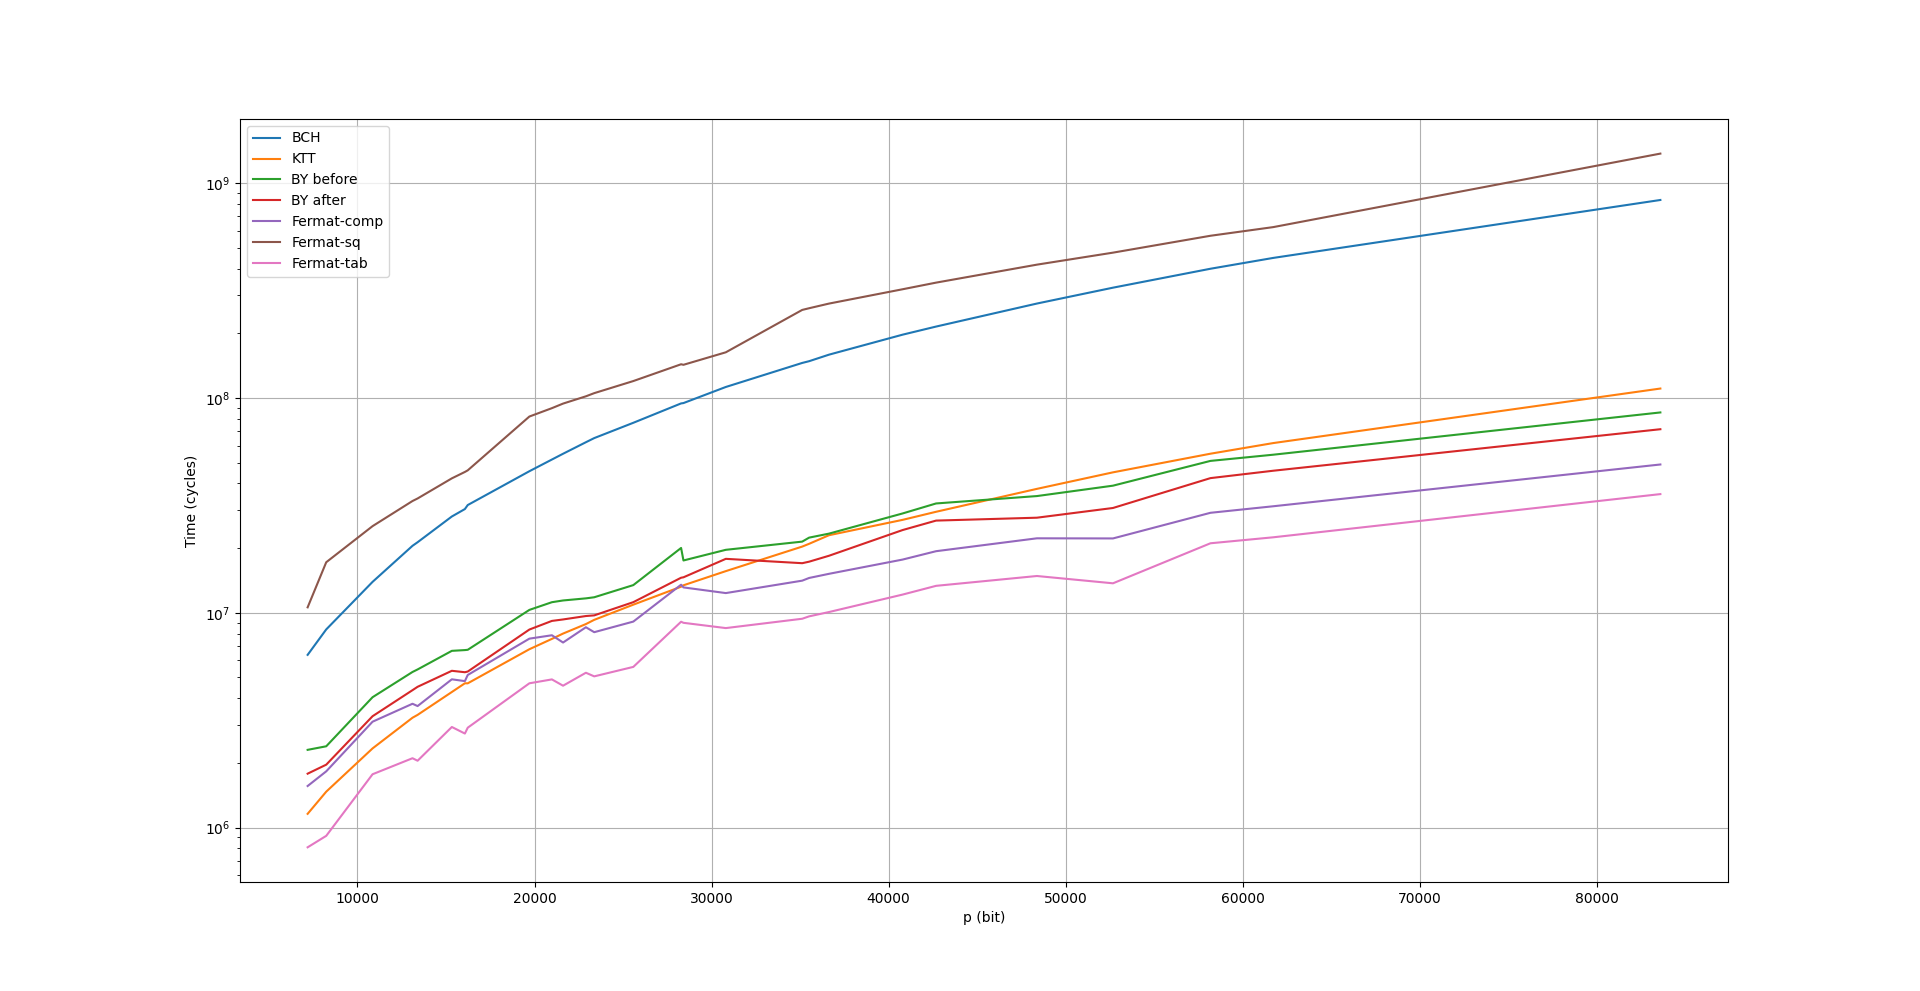
\includegraphics[width=\linewidth]{images/mean.png}
    \caption{Tempi di esecuzione}
\end{figure}
\begin{figure}
    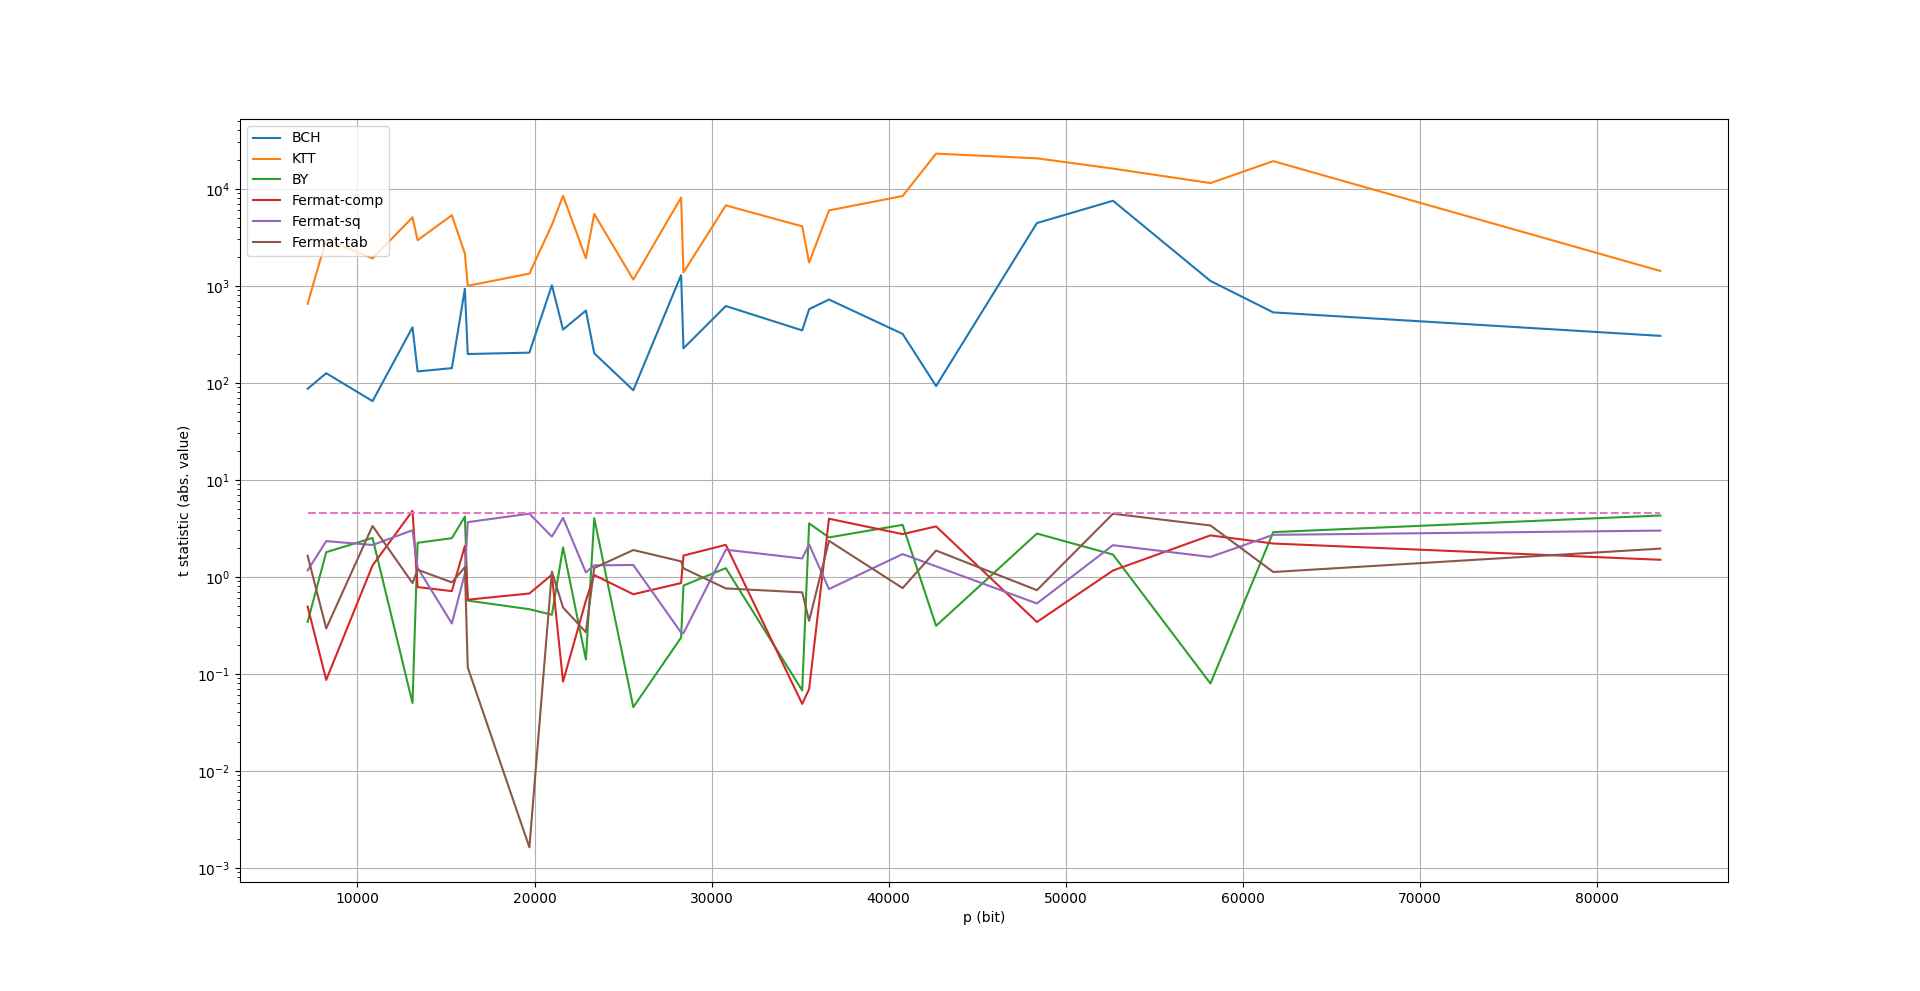
\includegraphics[width=\linewidth]{images/tstat.png}
    \caption{Valori della t statistica}
\end{figure}


Analizzando i risultati, notiamo che la \textit{nuova} versione dell'algoritmo di Bernstein-Yang ha un miglioramento
dal punto di vista temporale quasi costante per tutti i valori di $p$ (+18.56\%), rimanendo più lento dell'algoritmo
KTT~\cite{takagi2001fast} per $p < 35507$ (rispetto a $p < 48371$ della versione originale); d'altro canto, i valori della t di Student per BY sono inferiori in modulo a 4.5, la 
soglia sotto cui possiamo affermare che il tempo di esecuzione dell'algoritmo è indipendente dall'input con un
livello di confidenza del 99.999\%, a differenza di KTT. 




\bibliography{bib}

\end{document}
